\documentclass[border=4pt,class=socg-lipics-v2021]{standalone}
\usepackage{tikz}
\usetikzlibrary{calc}
\usetikzlibrary{patterns}
\usetikzlibrary{positioning}
\usetikzlibrary{decorations.pathreplacing}
%
\begin{document}%
\let\check\relax%
\centering%\setlength{\fboxsep}{0pt}\fbox{%
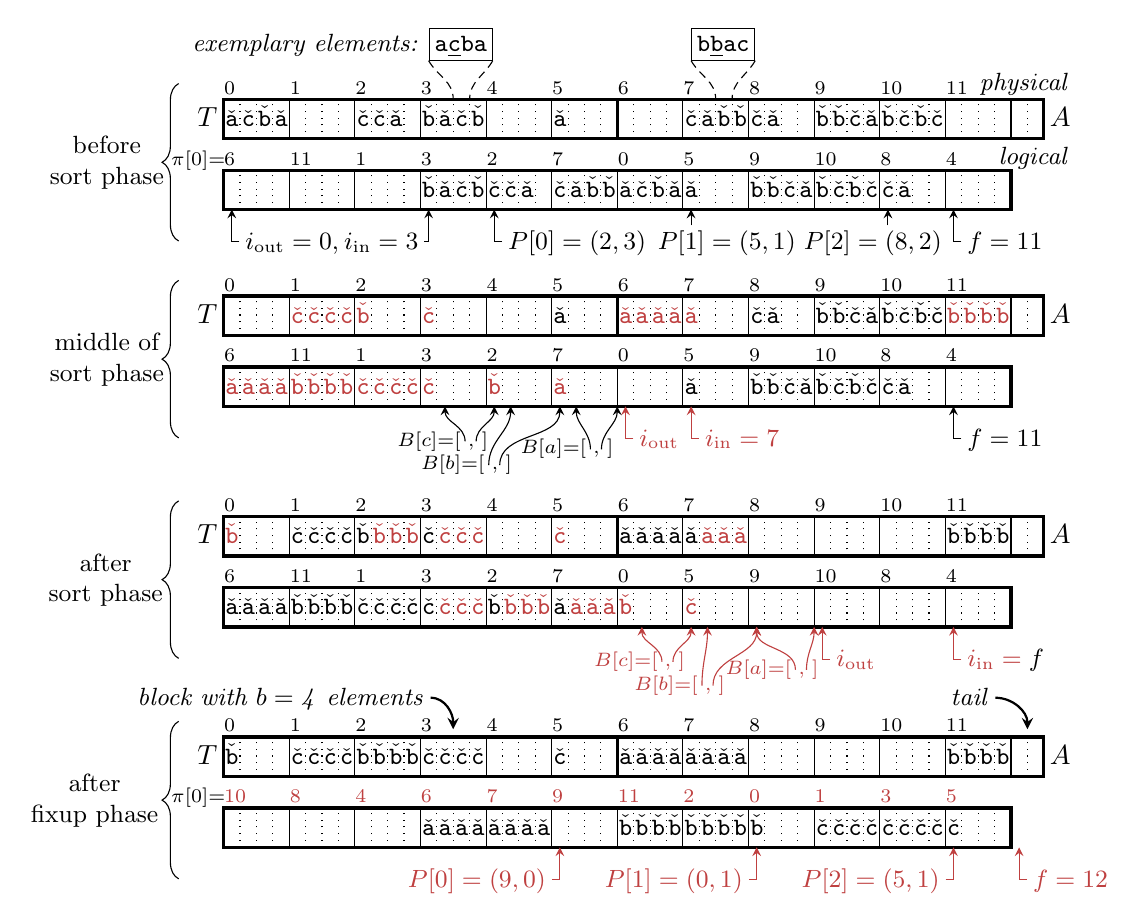
\begin{tikzpicture}
\def\mywidth{10}
%%  \node at (0,1) {$b = 2$};
%%  \node at (0,.5) {$\sigma = 3 = |\Sigma| = |\{\texttt{a}, \texttt{b}, \texttt{c}\}|$};
%%  \node at (0,0) {$A$};
%%  \node at (-1,0) {$T$};
%
  %%\node at (-4.2,-.5) {\texttt{---}};
  %%\node at (-3.5,-.5) {\texttt{---}};
  %%\node at (-2.8,-.5) {\texttt{---}};
  %%\node at (-2.1,-.5) {\texttt{---}};
  %%\node at (-1.4,-.5) {\texttt{---}};
  %%\node at (-.7,-.5) {\texttt{---}};
  %%\node at (0,-.5) {\texttt{abc}};
  %%\node at (.7,-.5) {\texttt{bca}};
  %%\node at (1.4,-.5) {\texttt{cab}};
  %%\node at (2.1,-.5) {\texttt{acb}};
  %%\node at (2.8,-.5) {\texttt{bac}};
  %%\node at (3.5,-.5) {$\cdots$};
  %%\node at (4.2,-.5) {\texttt{cba}};
%%
%%  \draw (0,0) rectangle (3,.5);
%\draw (-2,0) rectangle (11.8,.5);
%\node[anchor=west] at (-2,.2) {\small \texttt{acba xxxx ccax bacb xxxx axxx xxxx cabb caxx bbca bcbc xxxx}};
%\node[anchor=west] at (-2 ,-.5) {\small \texttt{xxxx xxxx xxxx bacb ccax cabb acba axxx bbaa bcbc caxx xxxx}};

% first physical array
\begin{scope}[font=\small, text height=1.5ex,text depth=.25ex,inner sep=2pt]
  \def\myyoffset{0}
  \draw (0,\myyoffset) rectangle +(\mywidth,.5);
  \foreach \c [count=\ci from 0] in
  {a,c,b,a,~,~,~,~,c,c,a,~,b,a,c,b,~,~,~,~,a,~,~,~,
   ~,~,~,~,c,a,b,b,c,a,~,~,b,b,c,a,b,c,b,c,~,~,~,~,~,~}
  {
    \if\c~{}\else
      {\node[xshift=3pt] at (\mywidth/48*\ci,\myyoffset+.25) {$\check{\texttt{\c}}$};}
    \fi
    \draw[dotted] (\mywidth/48*\ci,\myyoffset) -- +(0,.5);
  }

  % draw block of 4 separatpors
  \foreach \i in {4, 8, ..., 44}
    \draw (\mywidth/48*\i,\myyoffset) -- +(0,.5);
  \foreach \i in {0,1, 2, ..., 11}
    \node[anchor=south west,xshift=-2pt] at (\mywidth/48*\i*4,\myyoffset+0.45) {\scriptsize$\i$};

  % draw and annotate T and A boundaries
  \node[anchor=east] at (0,\myyoffset+.25) {\normalsize $T$};
  \draw[very thick] (0,\myyoffset) rectangle +(\mywidth/48*24,.5);
  \node[anchor=west] at (\mywidth/48*50,\myyoffset+.25) {\normalsize $A$};
  \draw[very thick] (\mywidth/48*24,\myyoffset) rectangle +(\mywidth/48*26,.5);

  \node[anchor=south east] at (\mywidth/48*50+.4,\myyoffset+.5) {\emph{physical}};
  \node[anchor=south east] at (\mywidth/48*50+.4,\myyoffset-.44) {\emph{logical}};

\end{scope}

% first virtual array
\begin{scope}[font=\small, text height=1.5ex,text depth=.25ex,inner sep=2pt]
  \def\myyoffset{-.9}
  \draw (0,\myyoffset) rectangle +(\mywidth,.5);
  \foreach \c [count=\ci from 0] in
  {~,~,~,~,~,~,~,~,~,~,~,~,b,a,c,b,c,c,a,~,c,a,b,b,
   a,c,b,a,a,~,~,~,b,b,c,a,b,c,b,c,c,a,~,~,~,~,~,~}
  {
    \if\c~{}\else
      {\node[xshift=3pt] at (\mywidth/48*\ci,\myyoffset+.25) {$\check{\texttt{\c}}$};}
    \fi
    \draw[dotted] (\mywidth/48*\ci,\myyoffset) -- +(0,.5);
  }

  % draw block of 4 separatpors
  \foreach \i in {4, 8, ..., 44}
    \draw (\mywidth/48*\i,\myyoffset) -- +(0,.5);
  \foreach \i [count=\ii from 0] in {6,11,1,3,2,7,0,5,9,10,8,4}
    \node[anchor=south west,xshift=-2pt] at (\mywidth/48*\ii*4,\myyoffset+0.45) {\scriptsize{$\i$}};

  % draw and annotate T and A boundaries
  %\node[anchor=east] at (0,\myyoffset+.25) {\normalsize $\pi[\cdot]$};
  \node[anchor=south east] at (.1,\myyoffset+.45) {\scriptsize $\pi[0]$=};
  \draw[very thick] (0,\myyoffset) rectangle +(\mywidth,.5);

  % draw pointers iout, iin and P[x]
  \node[anchor=north west,xshift=2mm] at (0,\myyoffset-.2) (iout) {$i_{\mathrm{out}}=0,$};
  \draw[->,>=stealth] (iout.west) -| (\mywidth/48/2,\myyoffset);

  \node[anchor=north west,xshift=1mm] at (\mywidth/48/2*13,\myyoffset-.2) (iin) {$i_{\mathrm{in}}=3$};
  \draw[->,>=stealth] (iin.east) -| (\mywidth/48/2*25,\myyoffset);

  \node[anchor=north west,xshift=1mm] at (\mywidth/48/2*33,\myyoffset-.2) (P0) {$P[0]=(2,3)$};
  \draw[->,>=stealth] (P0.west) -| (\mywidth/48/2*33,\myyoffset);

  \coordinate (Ptemp) at (\mywidth/48/2*57,\myyoffset-.2);
  \node[anchor=north west,xshift=-5mm] at (\mywidth/48/2*57,\myyoffset-.2) (P1) {$P[1]=(5,1)$};
  \draw[->,>=stealth] (P1.north -| Ptemp) -- (\mywidth/48/2*57,\myyoffset);

  \coordinate (Ptemp) at (\mywidth/48/2*81,\myyoffset-.2);
  \node[anchor=north west,xshift=0mm] at (\mywidth/48/2*70,\myyoffset-.2) (P2) {$P[2]=(8,2)$};
  \draw[->,>=stealth] (P2.north -| Ptemp) -- (\mywidth/48/2*81,\myyoffset);

  \node[anchor=north west,xshift=1mm] at (\mywidth/48/2*89,\myyoffset-.2) (F) {$f=11$};
  \draw[->,>=stealth] (F.west) -| (\mywidth/48/2*89,\myyoffset);

  % brace for the two arrays
  \path[draw,decorate,decoration={brace,raise=2pt,amplitude=6pt}]
    (-.5,\myyoffset-.4) -- +(0,2) node[pos=.6,left=5pt,text width=16mm,align=center,inner sep=0pt]{before sort phase};

% sample entries
  \node[draw,minimum width=8mm,anchor=west,node distance=-.4pt] at (\mywidth/48*28.5,1.2) (sampleentry) {\phantom{A}};
  \node[anchor=west] at (\mywidth/48*28.5,1.2) {\texttt{b\underline{b}ac}};
% zoom the block
\draw[densely dashed,black] (sampleentry.south west) to[out=300,in=90] (\mywidth/48*30,.5);
\draw[densely dashed,black] (sampleentry.south east) to[out=240,in=90] (\mywidth/48*31,.5);

  \node[draw,minimum width=8mm,anchor=west,node distance=-.4pt] at (\mywidth/48*12.5,1.2) (sampleentry) {\phantom{A}};
  \node[anchor=west] at (\mywidth/48*12.5,1.2) {\texttt{a\underline{c}ba}};
% zoom the block
\draw[densely dashed,black] (sampleentry.south west) to[out=300,in=90] (\mywidth/48*14,.5);
\draw[densely dashed,black] (sampleentry.south east) to[out=240,in=90] (\mywidth/48*15,.5);

  \node at (\mywidth/48*5,1.2) {\emph{exemplary elements:}};



\end{scope}








% middle physical array
\begin{scope}[font=\small, text height=1.5ex,text depth=.25ex,inner sep=2pt]
  \def\myyoffset{-2.5}
  \draw (0,\myyoffset) rectangle +(\mywidth,.5);
  % new entries
  \foreach \c [count=\ci from 0] in
  {~,~,~,~,c,c,c,c,b,~,~,~,c,~,~,~,~,~,~,~,~,~,~,~,
   a,a,a,a,a,~,~,~,~,~,~,~,~,~,~,~,~,~,~,~,b,b,b,b}
  {
    \if\c~{}\else
      {\node[xshift=3pt,red!50!gray] at (\mywidth/48*\ci,\myyoffset+.25) {$\check{\textbf{\texttt{\c}}}$};}
    \fi
    \draw[dotted] (\mywidth/48*\ci,\myyoffset) -- +(0,.5);
  }
  % old remaining entries
  \foreach \c [count=\ci from 0] in
  {~,~,~,~,~,~,~,~,~,~,~,~,~,~,~,~,~,~,~,~,a,~,~,~,
   ~,~,~,~,~,~,~,~,c,a,~,~,b,b,c,a,b,c,b,c,~,~,~,~,~,~}
  {
    \if\c~{}\else
      {\node[xshift=3pt] at (\mywidth/48*\ci,\myyoffset+.25) {$\check{\texttt{\c}}$};}
    \fi
    \draw[dotted] (\mywidth/48*\ci,\myyoffset) -- +(0,.5);
  }

  % draw block of 4 separatpors
  \foreach \i in {4, 8, ..., 44}
    \draw (\mywidth/48*\i,\myyoffset) -- +(0,.5);
  \foreach \i in {0,1, 2, ..., 11}
    \node[anchor=south west,xshift=-2pt] at (\mywidth/48*\i*4,\myyoffset+0.45) {\scriptsize$\i$};

  % draw and annotate T and A boundaries
  \node[anchor=east] at (0,\myyoffset+.25) {\normalsize $T$};
  \draw[very thick] (0,\myyoffset) rectangle +(\mywidth/48*24,.5);
  \node[anchor=west] at (\mywidth/48*50,\myyoffset+.25) {\normalsize $A$};
  \draw[very thick] (\mywidth/48*24,\myyoffset) rectangle +(\mywidth/48*26,.5);

\end{scope}

% middle virtual array
\begin{scope}[font=\small, text height=1.5ex,text depth=.25ex,inner sep=2pt]
  \def\myyoffset{-3.4}
  \draw (0,\myyoffset) rectangle +(\mywidth,.5);
  % new entries
  \foreach \c [count=\ci from 0] in
  {a,a,a,a,b,b,b,b,c,c,c,c,c,~,~,~,b,~,~,~,a,~,~,~,
   ~,~,~,~,~,~,~,~,~,~,~,~,~,~,~,~,~,~,~,~,~,~,~,~}
  {
    \if\c~{}\else
      {\node[xshift=3pt,red!50!gray] at (\mywidth/48*\ci,\myyoffset+.25) {$\check{\textbf{\texttt{\c}}}$};}
    \fi
    \draw[dotted] (\mywidth/48*\ci,\myyoffset) -- +(0,.5);
  }
  \foreach \c [count=\ci from 0] in
  {~,~,~,~,~,~,~,~,~,~,~,~,~,~,~,~,~,~,~,~,~,~,~,~,
   ~,~,~,~,a,~,~,~,b,b,c,a,b,c,b,c,c,a,~,~,~,~,~,~}
  {
    \if\c~{}\else
      {\node[xshift=3pt] at (\mywidth/48*\ci,\myyoffset+.25) {$\check{\texttt{\c}}$};}
    \fi
    \draw[dotted] (\mywidth/48*\ci,\myyoffset) -- +(0,.5);
  }

  % draw block of 4 separatpors
  \foreach \i in {4, 8, ..., 44}
    \draw (\mywidth/48*\i,\myyoffset) -- +(0,.5);
  \foreach \i [count=\ii from 0] in {6,11,1,3,2,7,0,5,9,10,8,4}
    \node[anchor=south west,xshift=-2pt] at (\mywidth/48*\ii*4,\myyoffset+0.45) {\scriptsize$\i$};

  % draw and annotate T and A boundaries
  %\node[anchor=east] at (0,\myyoffset+.25) {\normalsize $\pi[\cdot]$};
  \draw[very thick] (0,\myyoffset) rectangle +(\mywidth,.5);

  % draw pointers iout, iin and P[x]
  \node[anchor=north west,xshift=1mm,color=red!50!gray] at (\mywidth/48/2*49,\myyoffset-.2) (iout) {$i_{\mathrm{out}}$};
  \draw[->,>=stealth,color=red!50!gray] (iout.west) -| (\mywidth/48/2*49,\myyoffset);

  \node[anchor=north west,xshift=1mm,color=red!50!gray] at (\mywidth/48/2*57,\myyoffset-.2) (iin) {$i_{\mathrm{in}}=7$};
  \draw[->,>=stealth,color=red!50!gray] (iin.west) -| (\mywidth/48/2*57,\myyoffset);

  \node[anchor=north east,xshift=0mm] at (\mywidth/48/2*33,\myyoffset-.2) (Bc) {\scriptsize$B[c]$=[~,~]};
  \draw[->,>=stealth] ([xshift=-3.7mm,yshift=-1pt]Bc.east) to[out=90,in=270] (\mywidth/48/2*27,\myyoffset);
  \draw[->,>=stealth] ([xshift=-2.3mm,yshift=-1pt]Bc.east) to[out=90,in=270] (\mywidth/48/2*33,\myyoffset);


  \node[anchor=north east,xshift=3mm] at (\mywidth/48/2*33,\myyoffset-.5) (Bb) {\scriptsize$B[b]$=[~,~]};
  \draw[->,>=stealth] ([xshift=-3.7mm,yshift=-1pt]Bb.east) to[out=90,in=270] (\mywidth/48/2*35,\myyoffset);
  \draw[->,>=stealth] ([xshift=-2.3mm,yshift=-1pt]Bb.east) to[out=90,in=270] (\mywidth/48/2*41,\myyoffset);

  \node[anchor=north east,xshift=5.5mm] at (\mywidth/48/2*43,\myyoffset-.3) (Ba) {\scriptsize$B[a]$=[~,~]};
  \draw[->,>=stealth] ([xshift=-3.7mm,yshift=-1pt]Ba.east) to[out=90,in=270] (\mywidth/48/2*43,\myyoffset);
  \draw[->,>=stealth] ([xshift=-2.3mm,yshift=-1pt]Ba.east) to[out=90,in=270] (\mywidth/48/2*48,\myyoffset);

  \node[anchor=north west,xshift=1mm] at (\mywidth/48/2*89,\myyoffset-.2) (F) {$f=11$};
  \draw[->,>=stealth] (F.west) -| (\mywidth/48/2*89,\myyoffset);


%
%  \node[anchor=north west,xshift=1mm] at (\mywidth/48/2*81,\myyoffset-.2) (P2) {$P[2]=(8,2)$};
%  \draw[->,>=stealth] (P2.west) -| (\mywidth/48/2*81,\myyoffset);

  % brace for the two arrays
  \path[draw,decorate,decoration={brace,raise=2pt,amplitude=6pt}]
    (-.5,\myyoffset-.4) -- +(0,2) node[pos=.6,left=5pt,text width=16mm,align=center,inner sep=0pt]{middle of\\ sort phase};


\end{scope}










% lower physical array
\begin{scope}[font=\small, text height=1.5ex,text depth=.25ex,inner sep=2pt]
  \def\myyoffset{-5.3}
  \draw (0,\myyoffset) rectangle +(\mywidth,.5);
  % new entries
  \foreach \c [count=\ci from 0] in
  {b,~,~,~,~,~,~,~,~,b,b,b,~,c,c,c,~,~,~,~,c,~,~,~,
   ~,~,~,~,~,a,a,a,~,~,~,~,~,~,~,~,~,~,~,~,~,~,~,~}
  {
    \if\c~{}\else
      {\node[xshift=3pt,red!50!gray] at (\mywidth/48*\ci,\myyoffset+.25) {$\check{\textbf{\texttt{\c}}}$};}
    \fi
    \draw[dotted] (\mywidth/48*\ci,\myyoffset) -- +(0,.5);
  }
  % old remaining entries
  \foreach \c [count=\ci from 0] in
  {~,~,~,~,c,c,c,c,b,~,~,~,c,~,~,~,~,~,~,~,~,~,~,~,
   a,a,a,a,a,~,~,~,~,~,~,~,~,~,~,~,~,~,~,~,b,b,b,b,~,~}
  {
    \if\c~{}\else
      {\node[xshift=3pt] at (\mywidth/48*\ci,\myyoffset+.25) {$\check{\texttt{\c}}$};}
    \fi
    \draw[dotted] (\mywidth/48*\ci,\myyoffset) -- +(0,.5);
  }

  % draw block of 4 separatpors
  \foreach \i in {4, 8, ..., 44}
    \draw (\mywidth/48*\i,\myyoffset) -- +(0,.5);
  \foreach \i in {0,1, 2, ..., 11}
    \node[anchor=south west,xshift=-2pt] at (\mywidth/48*\i*4,\myyoffset+0.45) {\scriptsize$\i$};

  % draw and annotate T and A boundaries
  \node[anchor=east] at (0,\myyoffset+.25) {\normalsize $T$};
  \draw[very thick] (0,\myyoffset) rectangle +(\mywidth/48*24,.5);
  \node[anchor=west] at (\mywidth/48*50,\myyoffset+.25) {\normalsize $A$};
  \draw[very thick] (\mywidth/48*24,\myyoffset) rectangle +(\mywidth/48*26,.5);

\end{scope}

% lower virtual array
\begin{scope}[font=\small, text height=1.5ex,text depth=.25ex,inner sep=2pt]
  \def\myyoffset{-6.2}
  \draw (0,\myyoffset) rectangle +(\mywidth,.5);
  % new entries
  \foreach \c [count=\ci from 0] in
  {~,~,~,~,~,~,~,~,~,~,~,~,~,c,c,c,~,b,b,b,~,a,a,a,
   b,~,~,~,c,~,~,~,~,~,~,~,~,~,~,~,~,~,~,~,~,~,~,~}
  {
    \if\c~{}\else
      {\node[xshift=3pt,red!50!gray] at (\mywidth/48*\ci,\myyoffset+.25) {$\check{\textbf{\texttt{\c}}}$};}
    \fi
    \draw[dotted] (\mywidth/48*\ci,\myyoffset) -- +(0,.5);
  }
  \foreach \c [count=\ci from 0] in
  {a,a,a,a,b,b,b,b,c,c,c,c,c,~,~,~,b,~,~,~,a,~,~,~,
   ~,~,~,~,~,~,~,~,~,~,~,~,~,~,~,~,~,~,~,~,~,~,~,~}
  {
    \if\c~{}\else
      {\node[xshift=3pt] at (\mywidth/48*\ci,\myyoffset+.25) {$\check{\texttt{\c}}$};}
    \fi
    \draw[dotted] (\mywidth/48*\ci,\myyoffset) -- +(0,.5);
  }

  % draw block of 4 separatpors
  \foreach \i in {4, 8, ..., 44}
    \draw (\mywidth/48*\i,\myyoffset) -- +(0,.5);
  \foreach \i [count=\ii from 0] in {6,11,1,3,2,7,0,5,9,10,8,4}
    \node[anchor=south west,xshift=-2pt] at (\mywidth/48*\ii*4,\myyoffset+0.45) {\scriptsize$\i$};

  % draw and annotate T and A boundaries
  %\node[anchor=east] at (0,\myyoffset+.25) {\normalsize $\pi[\cdot]$};
  \draw[very thick] (0,\myyoffset) rectangle +(\mywidth,.5);

  % draw pointers iout, iin and P[x]
  \node[anchor=north west,xshift=1mm,color=red!50!gray] at (\mywidth/48/2*73,\myyoffset-.2) (iout) {$i_{\mathrm{out}}$};
  \draw[->,>=stealth,color=red!50!gray] (iout.west) -| (\mywidth/48/2*73,\myyoffset);

  \node[anchor=north west,xshift=1mm,color=red!50!gray] at (\mywidth/48/2*89,\myyoffset-.2) (iin) {$i_{\mathrm{in}}=\textcolor{black}{f}$};
  \draw[->,>=stealth,color=red!50!gray] (iin.west) -| (\mywidth/48/2*89,\myyoffset);

  \begin{scope}[color=red!50!gray]
  \node[anchor=north east,xshift=0mm] at (\mywidth/48/2*57,\myyoffset-.2) (Bc) {\scriptsize$B[c]$=[~,~]};
  \draw[->,>=stealth] ([xshift=-3.7mm,yshift=-1pt]Bc.east) to[out=90,in=270] (\mywidth/48/2*51,\myyoffset);
  \draw[->,>=stealth] ([xshift=-2.3mm,yshift=-1pt]Bc.east) to[out=90,in=270] (\mywidth/48/2*57,\myyoffset);


  \node[anchor=north east,xshift=3mm] at (\mywidth/48/2*59,\myyoffset-.5) (Bb) {\scriptsize$B[b]$=[~,~]};
  \draw[->,>=stealth] ([xshift=-3.7mm,yshift=-1pt]Bb.east) to[out=90,in=270] (\mywidth/48/2*59,\myyoffset);
  \draw[->,>=stealth] ([xshift=-2.3mm,yshift=-1pt]Bb.east) to[out=90,in=270] (\mywidth/48/2*65,\myyoffset);

  \node[anchor=north east,xshift=5.5mm] at (\mywidth/48/2*68,\myyoffset-.3) (Ba) {\scriptsize$B[a]$=[~,~]};
  \draw[->,>=stealth] ([xshift=-3.7mm,yshift=-1pt]Ba.east) to[out=90,in=270] (\mywidth/48/2*65,\myyoffset);
  \draw[->,>=stealth] ([xshift=-2.3mm,yshift=-1pt]Ba.east) to[out=90,in=270] (\mywidth/48/2*72,\myyoffset);
\end{scope}
% 72-48  +24
%
%  \node[anchor=north west,xshift=1mm] at (\mywidth/48/2*81,\myyoffset-.2) (P2) {$P[2]$=$(8,2)$};
%  \draw[->,>=stealth] (P2.west) -| (\mywidth/48/2*81,\myyoffset);

  % brace for the two arrays
  \path[draw,decorate,decoration={brace,raise=2pt,amplitude=6pt}]
    (-.5,\myyoffset-.4) -- +(0,2) node[pos=.6,left=4pt,text width=17mm,align=center,inner sep=0pt]{after\\ sort phase};

\end{scope}












% after fixup physical array
\begin{scope}[font=\small, text height=1.5ex,text depth=.25ex,inner sep=2pt]
  \def\myyoffset{-8.1}
  \draw (0,\myyoffset) rectangle +(\mywidth,.5);
  % old remaining entries
  \foreach \c [count=\ci from 0] in
  {b,~,~,~,c,c,c,c,b,b,b,b,c,c,c,c,~,~,~,~,c,~,~,~,
   a,a,a,a,a,a,a,a,~,~,~,~,~,~,~,~,~,~,~,~,b,b,b,b,~,~}
  {
    \if\c~{}\else
      {\node[xshift=3pt] at (\mywidth/48*\ci,\myyoffset+.25) {$\check{\texttt{\c}}$};}
    \fi
    \draw[dotted] (\mywidth/48*\ci,\myyoffset) -- +(0,.5);
  }

  % draw block of 4 separatpors
  \foreach \i in {4, 8, ..., 44}
    \draw (\mywidth/48*\i,\myyoffset) -- +(0,.5);
  \foreach \i in {0,1, 2, ..., 11}
    \node[anchor=south west,xshift=-2pt] at (\mywidth/48*\i*4,\myyoffset+0.45) {\scriptsize$\i$};

  % draw and annotate T and A boundaries
  \node[anchor=east] at (0,\myyoffset+.25) {\normalsize $T$};
  \draw[very thick] (0,\myyoffset) rectangle +(\mywidth/48*24,.5);
  \node[anchor=west] at (\mywidth/48*50,\myyoffset+.25) {\normalsize $A$};
  \draw[very thick] (\mywidth/48*24,\myyoffset) rectangle +(\mywidth/48*26,.5);

\end{scope}

% after fixup virtual array
\begin{scope}[font=\small, text height=1.5ex,text depth=.25ex,inner sep=2pt]
  \def\myyoffset{-9.0}
  \draw (0,\myyoffset) rectangle +(\mywidth,.5);
  \foreach \c [count=\ci from 0] in
  {~,~,~,~,~,~,~,~,~,~,~,~,a,a,a,a,a,a,a,a,~,~,~,~,
   b,b,b,b,b,b,b,b,b,~,~,~,c,c,c,c,c,c,c,c,c,~,~,~}
  {
    \if\c~{}\else
      {\node[xshift=3pt] at (\mywidth/48*\ci,\myyoffset+.25) {$\check{\texttt{\c}}$};}
    \fi
    \draw[dotted] (\mywidth/48*\ci,\myyoffset) -- +(0,.5);
  }

  % draw block of 4 separatpors
  \foreach \i in {4, 8, ..., 44}
    \draw (\mywidth/48*\i,\myyoffset) -- +(0,.5);
  \foreach \i [count=\ii from 0] in {10,8,4,6,7,9,11,2,0,1,3,5}
    \node[anchor=south west,xshift=-2pt,color=red!50!gray] at (\mywidth/48*\ii*4,\myyoffset+0.45) {\scriptsize$\i$};

  % draw and annotate T and A boundaries
  %\node[anchor=east] at (0,\myyoffset+.25) {\normalsize $\pi[\cdot]$};
  \node[anchor=south east] at (.1,\myyoffset+.45) {\scriptsize $\pi[0]$=};
  \draw[very thick] (0,\myyoffset) rectangle +(\mywidth,.5);

\begin{scope}[color=red!50!gray]
  % draw pointers P[x]
  \node[anchor=north east,xshift=-1mm] at (\mywidth/48/2*41,\myyoffset-.2) (P0) {$P[0]=(9,0)$};
  \draw[->,>=stealth] (P0.east) -| (\mywidth/48/2*41,\myyoffset);

  \coordinate (Ptemp) at (\mywidth/48/2*57,\myyoffset-.2);
  \node[anchor=north east,xshift=-1mm] at (\mywidth/48/2*65,\myyoffset-.2) (P1) {$P[1]=(0,1)$};
  \draw[->,>=stealth] (P1.east) -| (\mywidth/48/2*65,\myyoffset);

  \node[anchor=north east,xshift=-1mm] at (\mywidth/48/2*89,\myyoffset-.2) (P2) {$P[2]=(5,1)$};
  \draw[->,>=stealth] (P2.east) -| (\mywidth/48/2*89,\myyoffset);
\end{scope}

  \node[anchor=north west,xshift=1mm,color=red!50!gray] at (\mywidth/48/2*97,\myyoffset-.2) (F) {$f=12$};
  \draw[->,>=stealth,color=red!50!gray] (F.west) -| (\mywidth/48/2*97,\myyoffset);



%
%  \node[anchor=north west,xshift=1mm] at (\mywidth/48/2*81,\myyoffset-.2) (P2) {$P[2]=(8,2)$};
%  \draw[->,>=stealth] (P2.west) -| (\mywidth/48/2*81,\myyoffset);

\node at (\mywidth/48/2*7,\myyoffset+1.9) (block) {\emph{block with $b=\mathit4$ elements}};
  \draw[->,>=stealth,thick] (block.east) to[out=0,in=90] (\mywidth/48/2*28,\myyoffset+1.5);

\node at (\mywidth/48*45.5,\myyoffset+1.9) (endblock) {\emph{tail}};
  \draw[->,>=stealth,thick] (endblock.east) to[out=0,in=90] (\mywidth/48*49,\myyoffset+1.5);

  % brace for the two arrays
  \path[draw,decorate,decoration={brace,raise=2pt,amplitude=6pt}]
    (-.5,\myyoffset-.4) -- +(0,2) node[pos=.60,left=8pt,text width=17mm,align=center,inner sep=0pt]{after\\ fixup phase};

\end{scope}
%\node[rotate=20,color=gray!50!green] at (5,-4) {\Huge \textbf{\textsf{Work in Progress}}};
\end{tikzpicture}
%}% from fbox above for debugging
\end{document}
